\chapter{Implementation}
	The system must use Image Processing to get data from patterns via a webcam, send it to Unity and \textit{"translate"} it into a Virtual Reality garden that can be explored through the HTC Vive using Steam VR. There are many considerations to be made when developing a system like this. This section explains the program implementation and some of the algorithms that went into the development process. Furthermore, some of the most essential and relevant code snippets will also be presented.
	
	\section{Working in Unity}
The design was implemented in the Unity game engine\footnote{Unity's homepage \url{https://unity3d.com/}}. Unity allows high-level management of objects in space, which would greatly reduce development time on all the non-image processing aspects of developing the prototype.\todo{Why Unity as opposed to e.g. Unreal Engine?}

The SteamVR Unity plugin enabled an easy implementation of VR functionality in Unity. Moving and teleporting was achieved using standard scripts and assets included in the plugin. 	
The starting environment is simple, consisting of planes which make up the terrain and surrounding hedges. The image processing script developed for this project is attached to an invisible "Manager" object.
	\subsection{Implications of working with VR}

	Virtual Reality is computationally demanding. In 2016, graphics card manufacturer Nvidia estimated that an immersive VR experience was seven times more demanding than traditional PC gaming\footnote{venturebeat.com : \url{https://goo.gl/URA6R4}}. Nvidia got the number by combining the resolution needed for VR, 2 times 1680 x 1512, with the frame rate needed to avoid the adverse effect of VR, 90 fps. They compared the numbers with the same requirements for pc gaming 1920 x 1080, and 30 fps. However, this group agrees that 45 fps is closer to the minimum for a smooth experience\todo{Who is this group? The authors(us)? Based on what do we make this assessment?} , which still leaves the average laptop \todo{What is the average laptop? Sauce please} underpowered. At 45 fps, it has to render 2.5 times as many pixels, and twice as many frames per second compared to VR.
	For this reason the image processing algorithm should be quick to execute, as there is going to be a significant load on the system running the VR program. Consequently, work has been put into optimizing this algorithm.
	\todo{Any other consequences of VR? Price, development trouble?}
	\subsection{DLLs and Unity}
 		Unity has a number of different options for performing image processing. \todo{Then why are we developing our own markers instead of using Unity's functionality?} We would be creating the fiducial markers from scratch and could not use any preexisting software. At this point, we were already familiar with OpenCV, a fast library for image processing and computer vision, so developing using OpenCV made sense.\\
 		
		One challenge is that Unity uses C\# but OpenCV is only developed for C++, C, Python, and Java. The method used in this project to bridge this language barrier is to compile the C++ code as a DLL, or \textit{"Dynamic-link Library"}, and import it into the C\# code. DLLs cannot be executed in the way normal applications are, and are instead used by other applications. Because they can be compiled from a number of different languages they are not limited to what C\# code can do. Another advantage is that they are compiled in machine code and are therefore very fast\footnote{How to Write Native Plugins For Unity \url{https://www.alanzucconi.com/2015/10/11/how-to-write-native-plugins-for-unity/}}. There are some drawbacks to using DLLs as well, and these brought on some challenges during the implementation of the prototype. First, passing an object between the DLL and Unity is difficult because Unity cannot understand the same code as in the plug-in. On the DLL side you do not have a terminal, which means that getting any information about what is happening inside the DLL for debugging purposes is very problematic. For the same reason, debugging crashes is tricky, and the program would often crash without any feedback. \todo{Did we try to overcome this? Could we have?} Listing \ref{listing:dllExport} shows how to declare a function for export in C++.
\begin{listing}[H]
\caption{How to declare a function for DLL export in C++}
\label{listing:dllExport}
\begin{minted}[frame=lines, framesep=2mm,baselinestretch=1.1,fontsize=\footnotesize,linenos]{cpp}
extern "C" __declspec( dllexport ) int init(int w, int h);
\end{minted}
\end{listing}
\codeword{extern "C"} tells the compiler to not change the function's name, so that it can be imported into Unity. \codeword{__declspec()} tells the linker to act according to the argument, which in this case is \codeword{dllexport}. This lets the compiler know that it should export a function to a DLL. So now the function will be exported under a name that we know. In Unity a corresponding \codeword{DllImport("name")} will be used to import the function in Unity. Listing \ref{listing:dllImport} shows how this looks in C\# to be used by Unity.
\begin{listing}[H]
	\caption{How to declare a function for DLL import in C\#}
	\label{listing:dllImport}
	\begin{minted}[frame=lines,
	framesep=2mm,baselinestretch=1.1,fontsize=\footnotesize,linenos]{cpp}
[DllImport("unityOpencvPlugin", EntryPoint = "init")]
public static extern int Init(ref int outCameraWidth, ref int outCameraHeight);
	\end{minted}
\end{listing}
The name of the DLL file "unityOpencvPlugin" is given as an argument, and the function that we want to import is the "entrypoint". Unity will do a search for a function called \codeword{init} in the DLL "unityOpencvPlugin". Here it is important that the method names match completely, or it will not be found. In line 2, a function is declared that will call the imported method. Note that this function must have the same signature (return type and arguments) as the original. Unity can not check whether or not this is the case, so care must be taken to get it right. Signature compatibility is sensible for primitive types like \codeword{int}, but for objects it becomes a bit trickier. To do so requires declaration of similar objects in both languages, with variables in the same order, otherwise the data will not make sense when returned. In our case we need to return the position and rotational data of the markers found after image processing. They are represented in a structure like shown in Listing \ref{listing:objects}. 
\begin{listing}[H]
	\caption{Objects in C++ and C\#}
	\label{listing:objects}
	\begin{minted}[frame=lines, framesep=2mm,baselinestretch=1.1,fontsize=\footnotesize,linenos]{c++}
//in C++
struct ObjectData {
   int X, Y, Type, RotationX, RotationY, Rotation;
};

//in C#	
[StructLayout(LayoutKind.Sequential, Size = 16)]
public struct CVObject{
   public int X, Y, Type, RotationX, RotationY, Rotation;
}
	\end{minted}
\end{listing}
\todo{Does it make sense to have code from two different languages in the same code snippet?}
In Unity the structure needs to be laid out sequentially when exported to unmanaged memory\footnote{Unity layout \url{https://msdn.microsoft.com/en-us/library/system.runtime.interopservices.layoutkind(v=vs.110).aspx}}. \todo{What does it mean to have data laid out sequentially and what is unmanaged memory?} An object must be returned for each token. In this case it is easier to pass a pointer to an array, and make C++ fill it out from the code\todo{Needs more descriptive and "correct" terminology}. A few things are needed for this to work. The function needs to take a reference as an argument and the size of the array must be passed as an argument. Otherwise the function might try to access data outside of the array. The memory being referenced must also remain static or the pointer would no longer point to the right data. In C\# the keyword \codeword{Fixed} prevents data from being moved in memory, and \codeword{unsafe} enables working with pointers. In Listing \ref{listing:pointer} below there is an example from our implementation in the project where we pass a pointer to C++. %be careful with "unsafe" though. It oftentimes leads to children. 
\begin{listing}[H]
\caption{The function call to pass a pointer to C++, which is filled with object data by the code}
\label{listing:pointer}
\begin{minted}[frame=lines,
		framesep=2mm,baselinestretch=1.1,fontsize=\footnotesize,linenos]{c++}
unsafe{
	fixed (CVObject* outMarkers = _markers){
		Cap(outMarkers, _maxMarkerDetectCount, ref detectedMarkersCount);
	}
}
\end{minted}
\end{listing}


\section{BGR to RG chromaticity conversion}

A snap shot from the prototype's webcam is shown in \autoref{fig:snapshot}, and after each of the image processing sections, the output following this input will be shown.
\begin{figure}[H]
\centering
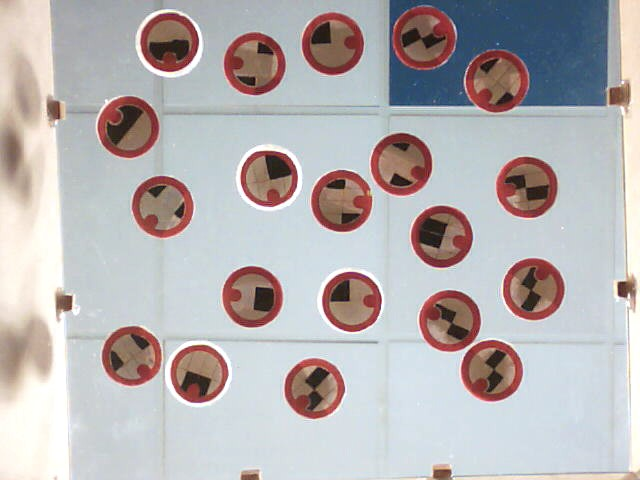
\includegraphics[width=0.6\linewidth]{figure/Analysis/testimage.jpg}
\caption{A test image ready for image processing}
\label{fig:snapshot}
\end{figure} 
OpenCV uses the BGR color format, which is like RGB with the order of colors changed.
It was found that differences in lighting conditions made thresholding the feed from the camera suboptimal. To circumvent this, the feed is converted to RG chromaticity\footnote{Wiki page for RG Chromaticity: \url{https://en.wikipedia.org/wiki/Rg_chromaticity}}, also known as normalized , and henceforth RG. RG contains no intensity information and as such is not a color space but rather a chromaticity space\footnote{Wiki page for Chromaticity: \url{https://en.wikipedia.org/wiki/Chromaticity}}. \todo{If we have extra time, find better source than wiki}
\subsection{Theory of RG}\label{sec:theoryOfRG}

The critical property of RG is that it does not record the individual channel's intensity, but rather the color's intensity as a percentage of the total intensity. Mathematically the RG value of a channel can be derived from an BGR value in the following way.
\begin{equation} 
 RG_x = \frac{BGR_x}{BGR_1 + BGR_2 + BGR_3}
\end{equation} 

Where $x$ represents which of the channels that is to be converted. This will return a value between 0 and 1 depending on how big a percentage of the total intensity comes from that particular color. Since floats are operationally slow, it is advised to scale the value to 8bits by multiplying by 255. So instead of operating on a range of 0.000 to 1.000, it operates on a range of 0 to 255. If one were to convert all three channels, with capital letter representing the RG chromaticity, the channels can be found as.
\begin{equation} 
RED = \frac{red}{red + blue + green} * 255
BLUE = \frac{blue}{red + blue + green} * 255
GREEN = \frac{green}{red + blue + green} * 255
\end{equation} 
This means that in RG the sum of all channels must be 255.
\begin{equation} 
\frac{red}{red + green + blue} + \frac{green}{red + green + blue} +  \frac{blue}{red + green + blue} =  \frac{red + green + blue}{red + green + blue} = 1
\end{equation} 
In RG, the channel values are codependent. If the value of red is large, then the other channels must by definition contain small values as they all must add up to 255. A result of this is that one can find the value in one channel if the other two are known.
\begin{equation} 
BLUE = 255 - RED - GREEN
\end{equation} 
So it is possible to store the data using two bits, and calculate the third color if it is needed. The loss of intensity data\cite{NormRGB} means a loss of information. For example, two colors (0,10,50) and (0,50,250) will produce exactly the same values when converted to RG.
\begin{equation} 
BLUE = \frac{50}{50 + 10} * 255 = (int)212.5 = 212 
BLUE = \frac{250}{250 + 50} * 255 = (int)212.5 = 212 
\end{equation} 
The resultant colors can be seen in \autoref{fig:conversion}. The same is true for any two colors that are proportionally similar.\\
\begin{figure}[H]
	\centering
	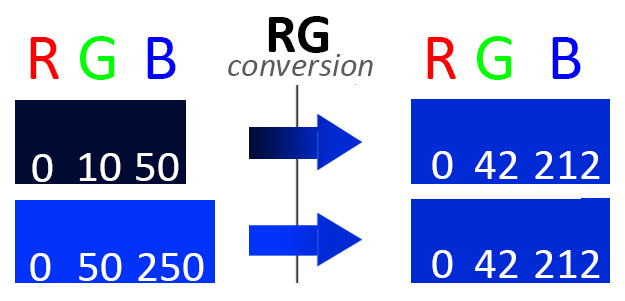
\includegraphics[width=0.6\linewidth]{figure/Analysis/rgconversion.png}
	\caption{Two colors of very different intensity are identical when converted to RG because they have the same percentages of the different colors. This make the RG color space more resistant to different lighting conditions}
	\label{fig:conversion}
\end{figure} 
In relation to image processing one has to be aware that noise, particularly in shadows, interfere with the RG space. For this reason it is recommended to zero the values if the total sum is below a certain value. \todo{sauce}

\subsection{RG chromaticity in code}
The process described above of converting a BGR image is a matter of point processing. We have made a few changes to the process to speed up the process at runtime. The current code performs these two steps for	 each pixel in the input image.\\
\begin{enumerate}
	\item Find the sum of the BGR channels.
	\item Assign the corresponding pixel in the output to the value found in a lookup table using the sum and value in the channel\\
\end{enumerate}
The only big change is the decision to use a lookup table. A lookup table is useful if you are going to be performing the same operation on similar data a lot of times. 
\subsection{Lookup tables}
A lookup table is a table in which the results of all possible inputs are calculated and stored. In the table one can look up what the result is, instead of calculating the same numbers every time\footnote{Wiki page for Lookup tables: \url{https://en.wikipedia.org/wiki/Lookup_table}}. In our case, this is necessary because of the magnitude of data we are working with. The webcam used had a resolution of 640 x 480. In total that is 307,200 pixels. Operations like multiplications, subtractions and additions are very fast, but division is a more computationally expensive operation\footnote{Streamhpc page on operation expenses: \url{https://streamhpc.com/blog/2012-07-16/how-expensive-is-an-operation-on-a-cpu/}} and division and multiplication operations are carried out three times per pixel (one for each channel). We found that at runtime, using a lookup table increased the speed of the RG conversion algorithm by 100.25\% as can be seen in table \ref{table:rgConvSpeed}.\\
\begin{multicols}{2}
	\begin{figure}[H]
	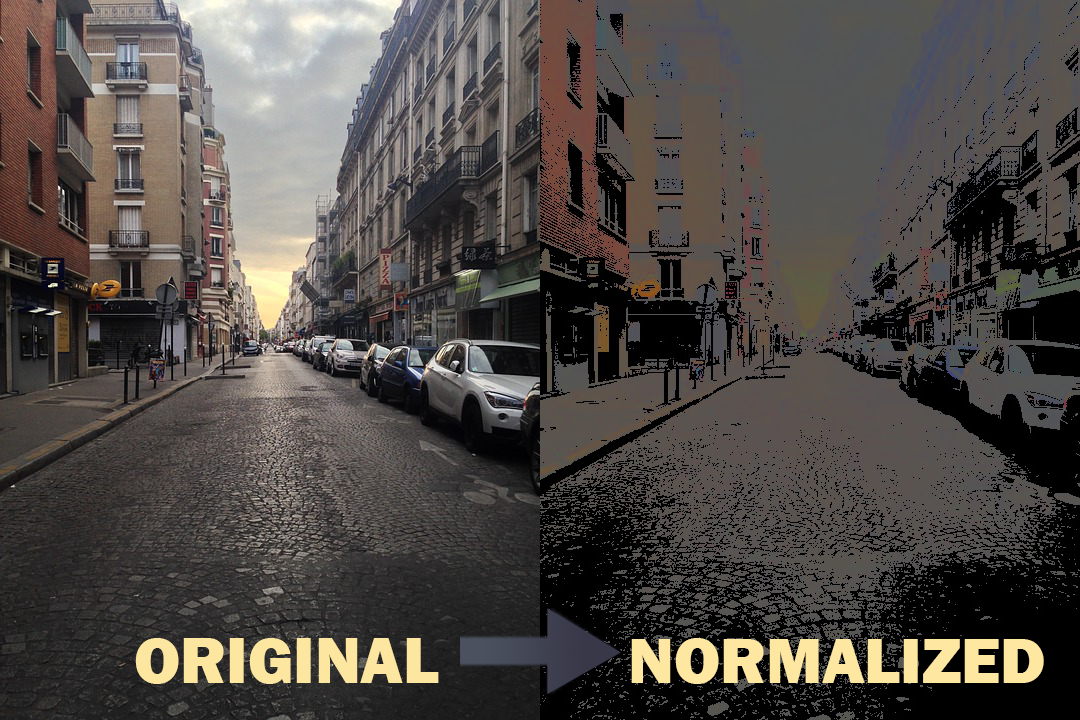
\includegraphics[width=1\linewidth]{figure/Analysis/Normalized.png}
	\label{rgConversion}
	\caption{Test image used to test the speed of the  RG conversion. Using a lookup table halved the execution time}
	\end{figure}

    \columnbreak
	\begin{table}[H]
		\centering
		\caption{Time taken to run the function. It can be seen that more data precomputed into a lookup table, results in faster execution. Due to the number of repetitions even something as basic as an "if less than" operation (As seen in line 4 of Listing \ref{listing:lutTable}) can significantly increase the time. Times are average times after 100,000 runs on a test image with the dimensions 540 * 720}
		\begin{tabular}{ l | l }
			\hline			
			No lookup table & .0015028 sec\\
			Lookup if above threshold & .0010218 sec\\
			Lookup table always& .0007741 sec\\
			\hline 
		\end{tabular}
	\label{table:rgConvSpeed}
	\end{table}
\end{multicols}

\todo{Why did we run the lookup table test on a random picture instead of a picture of markers, which would give a more accurate result?}

\subsection{Creating a lookup table}
To create a lookup table, the operation results for the full range of possible inputs are saved. We know from the theory section(See \autoref{sec:theoryOfRG}) that a color can be assigned by $RGcolor = 255 * \frac{color}{sumOfColor}$. There are two variables at play here. \textit{sumOfColor} which can vary between 0(all colors are 0), and 765(all colors are 255), and \textit{color} which can vary between 0, and 255. To compute a lookup table  that includes all possible combinations of variables, we need an array of size 766 * 256. The values are assigned when creating the table using a double for loop, shown in Listing \ref{listing:lutTable}.
\begin{listing}[H]
\caption{Instantiating our lookup table}
\label{listing:lutTable}
\begin{minted}[frame=lines,
	framesep=2mm,baselinestretch=1.1,fontsize=\footnotesize,linenos]{c++}
int divLUT[766][256]; //division lookuptavle;
for (int i = 0; i < 766; i++) {
   for (int j = 0; j < 256; j++) {
      if (i < rgConvThreshold) { 
         divLUT[i][j] = 0;
      } else {
         divLUT[i][j] = (j * 255) / i;
      }
   }
}
\end{minted}
\end{listing}
The first thing the loop does is to check if the arguments are below the threshold where they should be zeroed (to prevent noise in dark areas from messing with the image). In that case it sets the index to zero. Otherwise it calculates the value that would result from the color \codeword{j} divided by sum \codeword{i} and multiplied by 255.
\subsubsection{Summing BGR channels and looking up results}
To use the lookup table we have to visit each pixel once and look up the value in the pixel. This is done using a double for loop. Our implementation, seen in Listing \ref{listing:sum}, takes an input image assumed to be BGR, an output image also assumed to be BGR, and a reference to the table. The ampersand \codeword{&} in the function signature indicates that the argument should be passed by reference. This allows for changes to the original data to be made. If not included we would be making changes to copies instead.\todo{What's the benefit of changing the original data instead of just making a copy?} \\
\begin{listing}[H]
	\caption{RG conversion code}
	\label{listing:sum}
	\begin{minted}[frame=lines,
	framesep=2mm,baselinestretch=1.1,fontsize=\footnotesize,linenos]{c++}
	void preLookUpBgr2rg(Mat &in, Mat &out, uchar (&divLUT)[766][256]) {
	//declare other variables
	int nCols = in.cols * 3;	//since there's 3 channels per pixel
	
	for (int i = 0; i < nRows; i += GRIDSIZE) {
	p = in.ptr<uchar>(i);
	cp = out.ptr<uchar>(i);
	
	for (int j = 0; j < nCols; j += 3 * GRIDSIZE) {
		blue = p[j];
		green = p[j+1];
		red = p[j+2];
		sum = blue + green + red;
		lutptr = divLUT[sum];
		//cp[j] = *(lutptr + blue);  not needed
		cp[j + 1] = *(lutptr + green);
		cp[j + 2] = *(lutptr + red);
		}
	}
}
	\end{minted}
\end{listing}
Before the loop we instantiate three pointers so we don't have to instantiate them inside the loop. \codeword{p} is a pointer to a row in the BGR image we want to convert. \codeword{cp} is a pointer to the equivalent row in the output image. \codeword{lutptr} points to a row in the lookup table. This is useful because the sum, and therefore the column, will be the same for each color in the pixel. So we will be looking at the same column three times in a row, one for blue, one for green and one for red. With the pointers the program will not need to jump as far in memory every time the lookup table is used. It is quicker to get from \codeword{lutptr[sum][0]} to \codeword{lutptr[sum][red]}, than from codeword{lutptr[0][0] to \codeword{lutptr[sum][red]}. This can be seen in Figure \ref{fig:table}.
\begin{figure}[H]
	\centering
	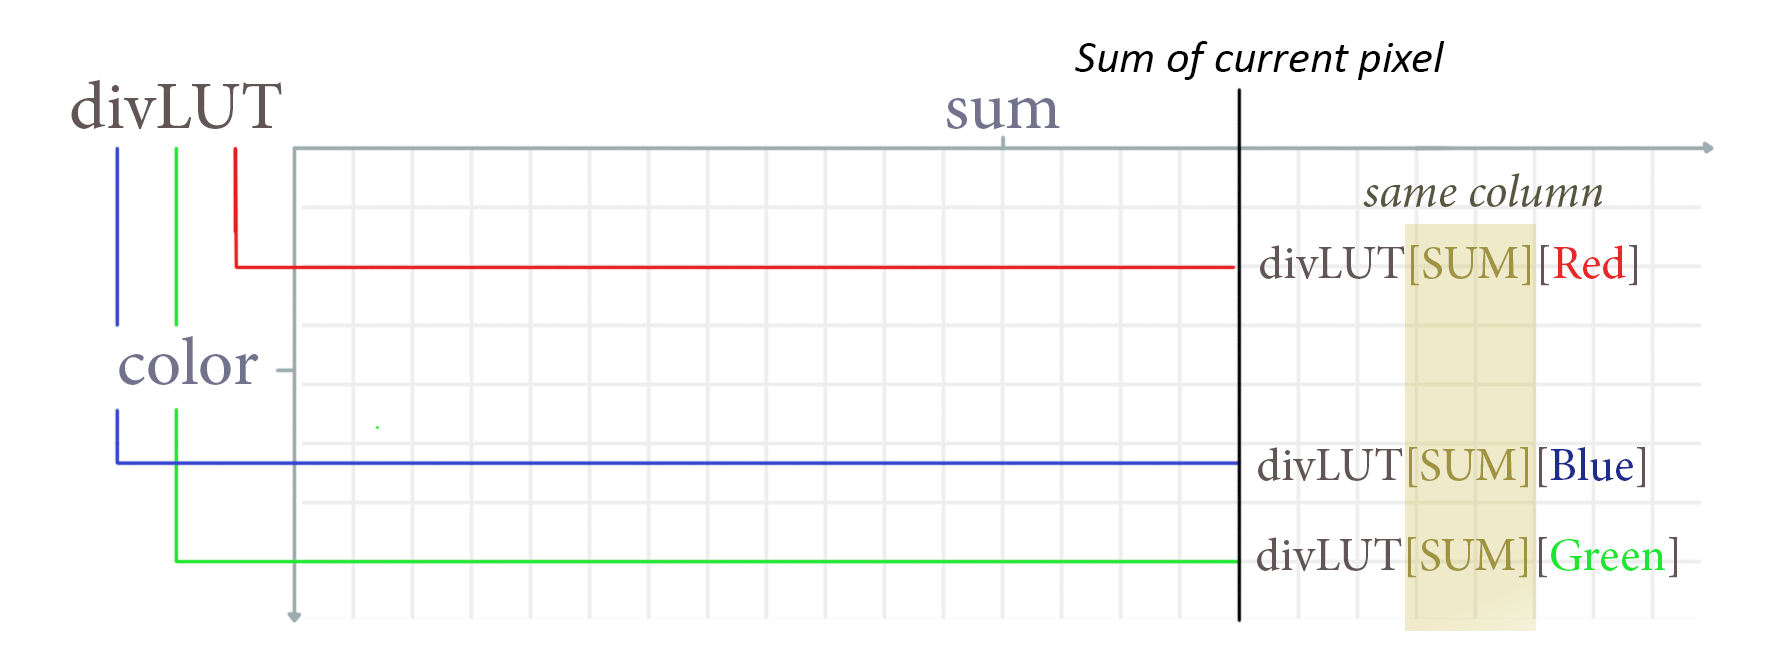
\includegraphics[width=0.9\linewidth]{figure/Analysis/table.png}
	\caption{Demonstration of why the column is the same in the lookup of all three colors. The sum of the pixel color does not change, and neither does the column.}
	\label{fig:table}
\end{figure} 
Inside the for loop, the code starts by saving the values of each channel to the corresponding variables. The values are then added together. Now we have the two variables that we need to use the lookup table. Since the sum is not going to change we get the address of the row of the sum and save it in \codeword{lutptr}. Now we can assign the values using \codeword{lutptr}. In accordance with the theory section(See \autoref{sec:theoryOfRG}) blue is unnecessary data and so does not need to be assigned. We will be calculating the blue when showing the output, but that is only to make the image less jarring for humans to look at. In the final code it can be omitted. After executing the function on our test image the following \autoref{fig:rgsnapshot} is the output.
\begin{figure}[H]
	\centering
	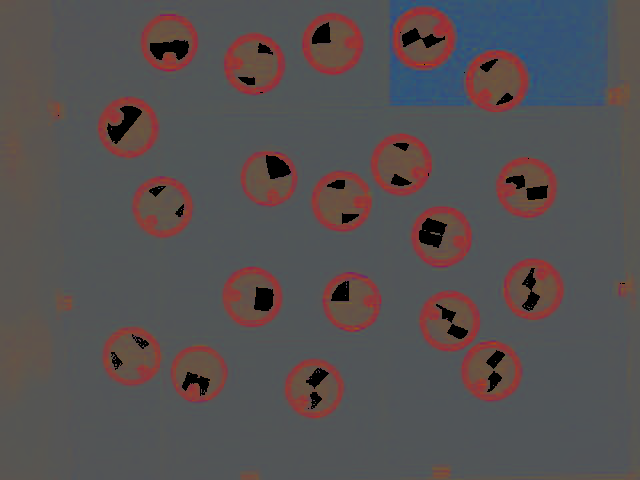
\includegraphics[width=0.6\linewidth]{figure/Analysis/rgbNorm.png}
	\caption{Test image after being converted into RG}
	\label{fig:rgsnapshot}
\end{figure} 

\section{Thresholding in RG}
Because RG can be represented by two values it is possible to plot the  chromaticity space using two axes, as can be seen in \autoref{fig:rgbNorm}. The image shows a slightly modified RG space. 
\begin{figure}[H]
	\centering
	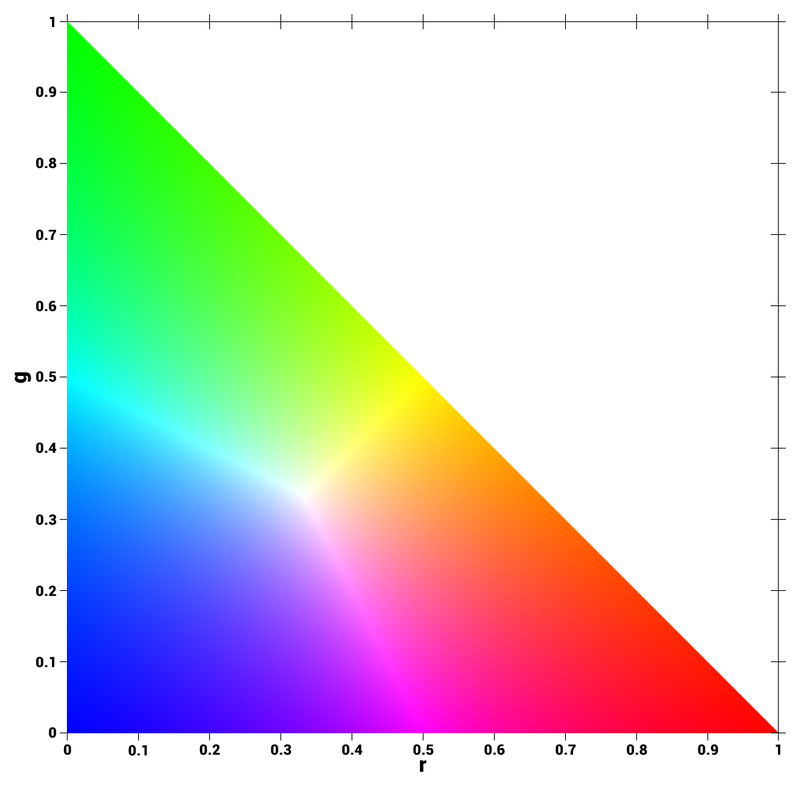
\includegraphics[width=0.5\linewidth]{figure/Analysis/normRGB.png}
	\caption{The entire RG color space is visible here, it can be represented in 2D due to the lack of intensity data\protect\footnotemark}
	\label{fig:rgbNorm}
\end{figure}
\footnotetext{\url{https://en.wikipedia.org/wiki/Rg\_chromaticity}, made by Vampyrium, and will be used to illustrate the results of different thresholds. Under the CC BY-SA 3.0 license.}
There are different ways to threshold in RG. Common among all of the presented approaches is that they use the red and green values of each pixel to determine whether the pixel should be set to 255
or 0.\\

\textbf{In Range} is a method of thresholding in the HSV color space\footnote{openCV tutorial where inRange() is used: \url{https://docs.opencv.org/3.2.0/df/d9d/tutorial\_py\_colorspaces.html}}. A range is defined on each axis in which to threshold. For example between 160 to 255 in red, and 0 to 60 in green. The thresholding consists of comparing the red and green value in each pixel to the ranges. If both values are inside the designated range the pixel is set to 255, else it is set to 0. The resulting threshold can be seen in \autoref{thresholdintrange}. This will create a square segmentation in the chromaticity space because we are comparing two constants which create straight lines. With its square shape, it can be difficult to get a broad enough spectrum, without cutting into different colors. For example, under blue light from the sky the markers might be a bit bluer. It also cannot be set too wide, since doing so will cause white elements to also be segmented. There are, however, ways the provide more control over the segmentation.\\

	\begin{figure}[H]
		\begin{minipage}[b]{0.49\textwidth}
		\centering
		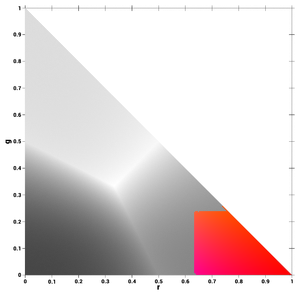
\includegraphics[width=1\linewidth]{figure/Analysis/inrangethresholdcolor.png}
		\caption{In Range threshold in RG space}
		\label{thresholdintrange}
	
	\end{minipage}
	\hfill
	\begin{minipage}[b]{0.49\textwidth}

		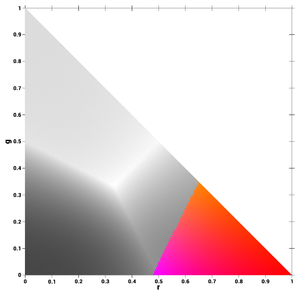
\includegraphics[width=1\linewidth]{figure/Analysis/belowlinethresholdthresholdcolor.png}
		\caption{Below line threshold in RG space}
		\label{fig:thresholdbelowline}
	\end{minipage}
	\end{figure}
	


\textbf{Line threshold}. Another potential way to threshold is to use a line treshold. One creates a straight line with a formula $y = ax - b$. Where y and x each represent the two axes. $a$ determines the slope of the line and is controlled by $x$ which is one of the colors. If $x$ is red, then $b$ determines where the thresholding should start and can be found using $b =- i * a$, where $i$ is the starting point of the line. Based on the equation we can find value of green that would place it on the line for a given red value. It is then determined on which side of the line the values lie. If the values are on the right side it is set to 255, else it is set to zero. A below line threshold is seen in \autoref{fig:thresholdbelowline}\\
\begin{multicols}{2}
	\begin{figure}[H]
		\centering
		\label{thresholddist}
		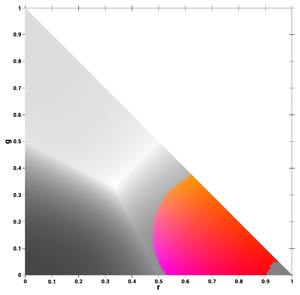
\includegraphics[width=1\linewidth]{figure/Analysis/distthresholdcolor.png}
		\caption{distance threshold in rg space}
	\end{figure}
	
	\begin{figure}[H]
		\centering
		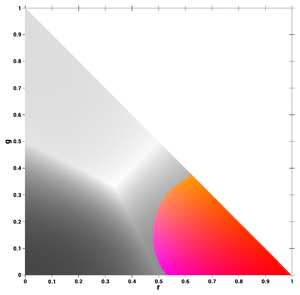
\includegraphics[width=1\linewidth]{figure/Analysis/thresholdcolor.png}
		\caption{combined threshold in rg space}
		\label{fig:threshold}
	\end{figure}	
\end{multicols}
\todo{These figures should have full color}
\textbf{Distance threshold} Distance tresholding is based on finding the chromaticity distance from a pixel's color to a reference value in RG. If the distance is below a threshold the set it to 255, else 0. In two dimensions, the distance between two points $p_0$ and $p_1$ can be found as $d = \sqrt{(p_1x - p_0x)^2 +(p_1y - p_0y)^2}$. In our implementation we used a distance threshold with a red value of 180 and a green value of 40 for our reference color. The threshold distance was set to 60. This produces the threshold observed in \autoref{fig:threshold}. This works well for the purposes of the project, but doesn't allow for the tresholding of extremely red color, as a circle of that size and position does not cover the lower right corner of the RG space. \\

\textbf{Combined Threshold}. It is possible to combine these different approaches to thresholding. Combining and subtracting the thresholds allows shaping the treshold to suit any need. Following the problems with segmenting extreme reds, we decided to add an In Range to the Distance Threshold to ensure that we could capture all the shades of red. The resulting threshold can be seen in \autoref{fig:threshold}. This produces the most consistent threshold for the prototype, as it is very resistant to lighting changes.

\subsection{Thresholding implementation}
Like the RG conversion, this operation involves visiting each pixel once and performing an operation that uses its color values as inputs. A lookup table is used here. First, the distance is found. If it is smaller than the threshold, the pixel is set to 255, else, set it to 0. Listing \ref{listing:thresholdDist} shows how we initialized our table.

\begin{listing}[H]
	\caption{Instantiating the Distance threshold lookup table}
	\label{listing:thresholdDist}
	\begin{minted}[frame=lines,
framesep=2mm,baselinestretch=1.1,fontsize=\footnotesize,linenos]{c++}
uchar lookup[256][256];
for (int i = 0; i < 256; i++) {
	for (int j = 0; j < 255; j++) {
		if (j > 180) { // if red is above 180
			lookup[i][j] = 255;
		} else if (((i - g)*(i - g) + ((j - r)*(j - r))) < 3600) {
			lookup[i][j] = 255;
		} else {
			lookup[i][j]= 0;
		}
	}
}
\end{minted}
\end{listing}

\todo{Explain why we use uchar}
Inside the double for loop there are two if statements that each perform a different thresholding operation. The first is an In Range where it checks if the red color is larger than 180. The second is checks the distance from the inputs $f(j,i)$ to a reference point $p(r,g)$. Rather than comparing it to the distance, it compares to the distance squared. This removes the need to calculate the square root, which is a computationally expensive operation. A check is made for whether the distance is smaller than 60. If either of these if statements are true, the index is made white, otherwise it is made black.
In terms of implementation using the lookup table, it is very similar to the RG conversion. The output after thresholding the normalized test image, can be seen in \autoref{fig:thsnapshot}\\
\begin{figure}[H]
	\centering
	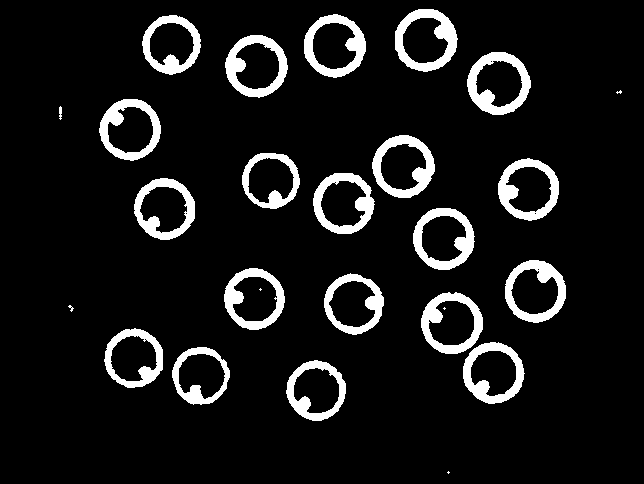
\includegraphics[width=0.6\linewidth]{figure/Analysis/thresholded.png}
	\caption{The thresholded version of the normalized test image}
	\label{fig:thsnapshot}
\end{figure} 
The algorithm has now produced a binary thresholded image with values that are either 255 or 0. A grassfire blob detection will be performed on this image. 
\section{Blob detection}
Blob detection is used to segment a picture into individual blobs. If you need to deal with multiple objects in a image, it is worth investigating. 
\subsection{What is a blob, and why detect them}
BLOB stands for \textbf{B}inary \textbf{L}arge \textbf{OB}ject. They represent regions of interest (ROI) in an image. Extracting the blobs from an image can significantly cut down on processing time, because the program now only have to process the ROI instead of the entire image. Another use is to calculate features that might be useful to know about the blob like size, bounding box, and others. For a program trying to recognize real life objects, knowing the range of features that the object normally exhibits can help it determine if a blob is like that object. These features are calculated from the list of pixels which the blob consists of.\\

There is a large amount of features that could be calculated from a blob. But our job is made a lot easier by three factors. First, our markers are resting on a surface perpendicular to the camera. This means that rotation will only happen in two dimensions and that the shape of the markers will not change substantially when rotated. Secondly, our markers are circles. Circles have many advantages. Their height/width relationship is the same in any rotation, and you can work with its radius. Finally, we are segmenting based on a bright distinctive color(red), meaning that the thresholded version of the image contains just the regions of interest(See \autoref{fig:thsnapshot}). This makes the blob detection very accurate.
\subsection{The blob object and parameters}
The list of pixels and blob parameters are often held in an structure.
We created one for this purpose. Our blob structure is called \codeword{glyphObj} because the pattern underneath can be considered a glyph\footnote{\url{AForge Article on Glyphs' recognition: http://goo.gl/HkFksM}}. The structure is declared as shown in listing \ref{listing:glyph}
\begin{listing}[H]
	\caption{The declaration of glyph object, the structure that contain a blob, as well has the parameters about it}
	\begin{minted}[frame=lines, framesep=2mm,baselinestretch=1.1,fontsize=\footnotesize,linenos]{c++}
struct glyphObj {
	vector<cVector> list;
	cVector bBoxStart;
	cVector bBowEnd;
	cVector center;
	cVector rotation;
	int nr;
	bool returnable = false;
};
	\end{minted}
	\label{listing:glyph}
\end{listing}
The parameters and what they are used for will be explained in detail in the next section, so the uses of the variables will be not be covered extensively here. However, here is a brief overview:
cVector is short for coordinate vector and contains two integers, one for each of the dimensions. In C++ a vector is a list type that can grow dynamically. So the vector of cVectors is going to contain the coordinates of all the pixels in the blob. bBox is short for bounding box and holds the two coordinates used to draw a bounding box around the blob, and find its height to width ratio. Since a circle always has similar height to width ratio in any rotation, this parameter can be used to disqualify a lot of false blobs. \codeword{center} is the coordinates to the center of the bounding box.
The integer \codeword{nr} is used to help visualize the grass-fire algorithm, and will later contain the found numerical value from the pattern underneath the markers. Finally, since the program finds more blobs than there are actual markers, and returning all the blobs to Unity is suboptimal, a boolean variable \codeword{returnable} is used. It is only set to true if the blob passes all tests and therefore is considered a marker.

\subsection{Blob Extraction by recursion}
All features of a blob are calculated from a list of pixels included in it. This section deals with how to get that initial list of pixels. In a segmented image, a blob is a number of neighboring white pixels. Each pixel in the blob must be connected to all the others. Therefore, a blob can be found by discovering all connected pixels of any one pixel in the blob.\\

The process of extracting a blob is as follows. A pixel is found, and is now treated as a new blob. If any pixels that it shares borders with it are white, they are added to the blob. Their neighbors are now checked for white pixels, and so the process continues recursively. To ensure that each pixel is added to the blob only once, adding a pixel to the blob should change its color. When no more connected pixels can be found, the blob is finished. A new, unconnected white pixel is then found, and the process starts again. The new color for pixels added to a blob ensures that no pixels from the first blob will be found.\\
This process is called a grassfire algorithm, because it starts at a point, spreads like a fire in all directions, and dies when there are no more pixels to "burn".
It is a recursive algorithm. This recursive function call is simple to implement but means that the program's call stack might fill up and crash it, a concept illustrated metaphorically in \autoref{fig:firefighter}.  \todo{what is a call stack}
\begin{figure}[H]
	\centering
	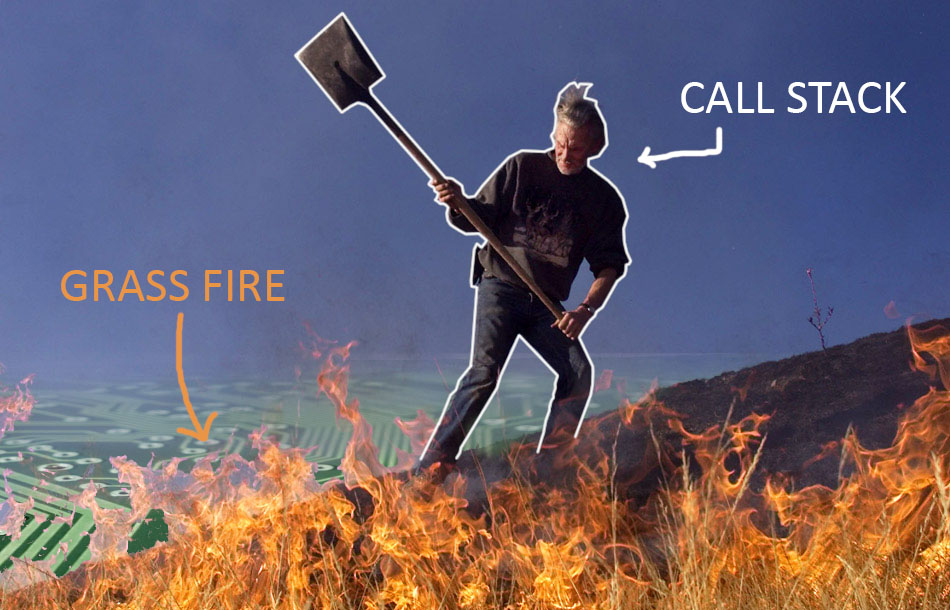
\includegraphics[width=0.6\linewidth]{figure/Analysis/firefighter.jpg}
	\caption{What happens inside your call stack during a grassfire algorithm. The fire spreads adding calls onto the stack, raging out of control, putting our call stack, the old man, in danger. Until the fire is done spreading the stack cannot resolve. When done spreading the call stack is resolved, represented by the old man, can out the fire.}
	\label{fig:firefighter}
\end{figure} 
\todo{If the fire is literally out of control, why is the man fighting it? The fire stops itself when there is no more to burn}
Due to the relatively small blobs in our program, usually between 150 and 450 pixels in area, a stack overflow could be prevented by increasing the stack heap size to 4 MB from 1 MB. However, larger resolutions would cause significantly bigger issues. If we double the number of pixel in each axis, we get a four times larger blob. At large resolutions, the stack would have to be larger to accommodate the recursive function. Sampling that many pixels would also slow down the algorithm. While the webcam used in the prototype had a small resolution, larger resolutions were considered for the final prototype during early stages of development. A variable called \codeword{gridSize} was added to alleviate the problem. It causes the algorithm to make jumps of \codeword{gridSize} pixels instead of 1. Instead of checking the pixel immediately to the right, the algorithm will check the one \codeword{gridSize} places to the right. Setting \codeword{gridSize} to 2 will cause the blobs to be four times as small, solving the problem caused by a larger camera resolution. Now the algorithm's speed and accuracy can be tailored to suit the specific need.
\subsection{Grassfire implementation}
Our implementation can be seen in Listing \ref{listing:grassfireIm}. Due to its recursive nature, this method will be called many thousands of times. Note that the function does not make use of the very computationally expensive \codeword{Mat.at<uchar>(y,x)}} function. Instead pointers are used to navigate both horizontally and vertically.
\begin{figure}[H]
	\centering
	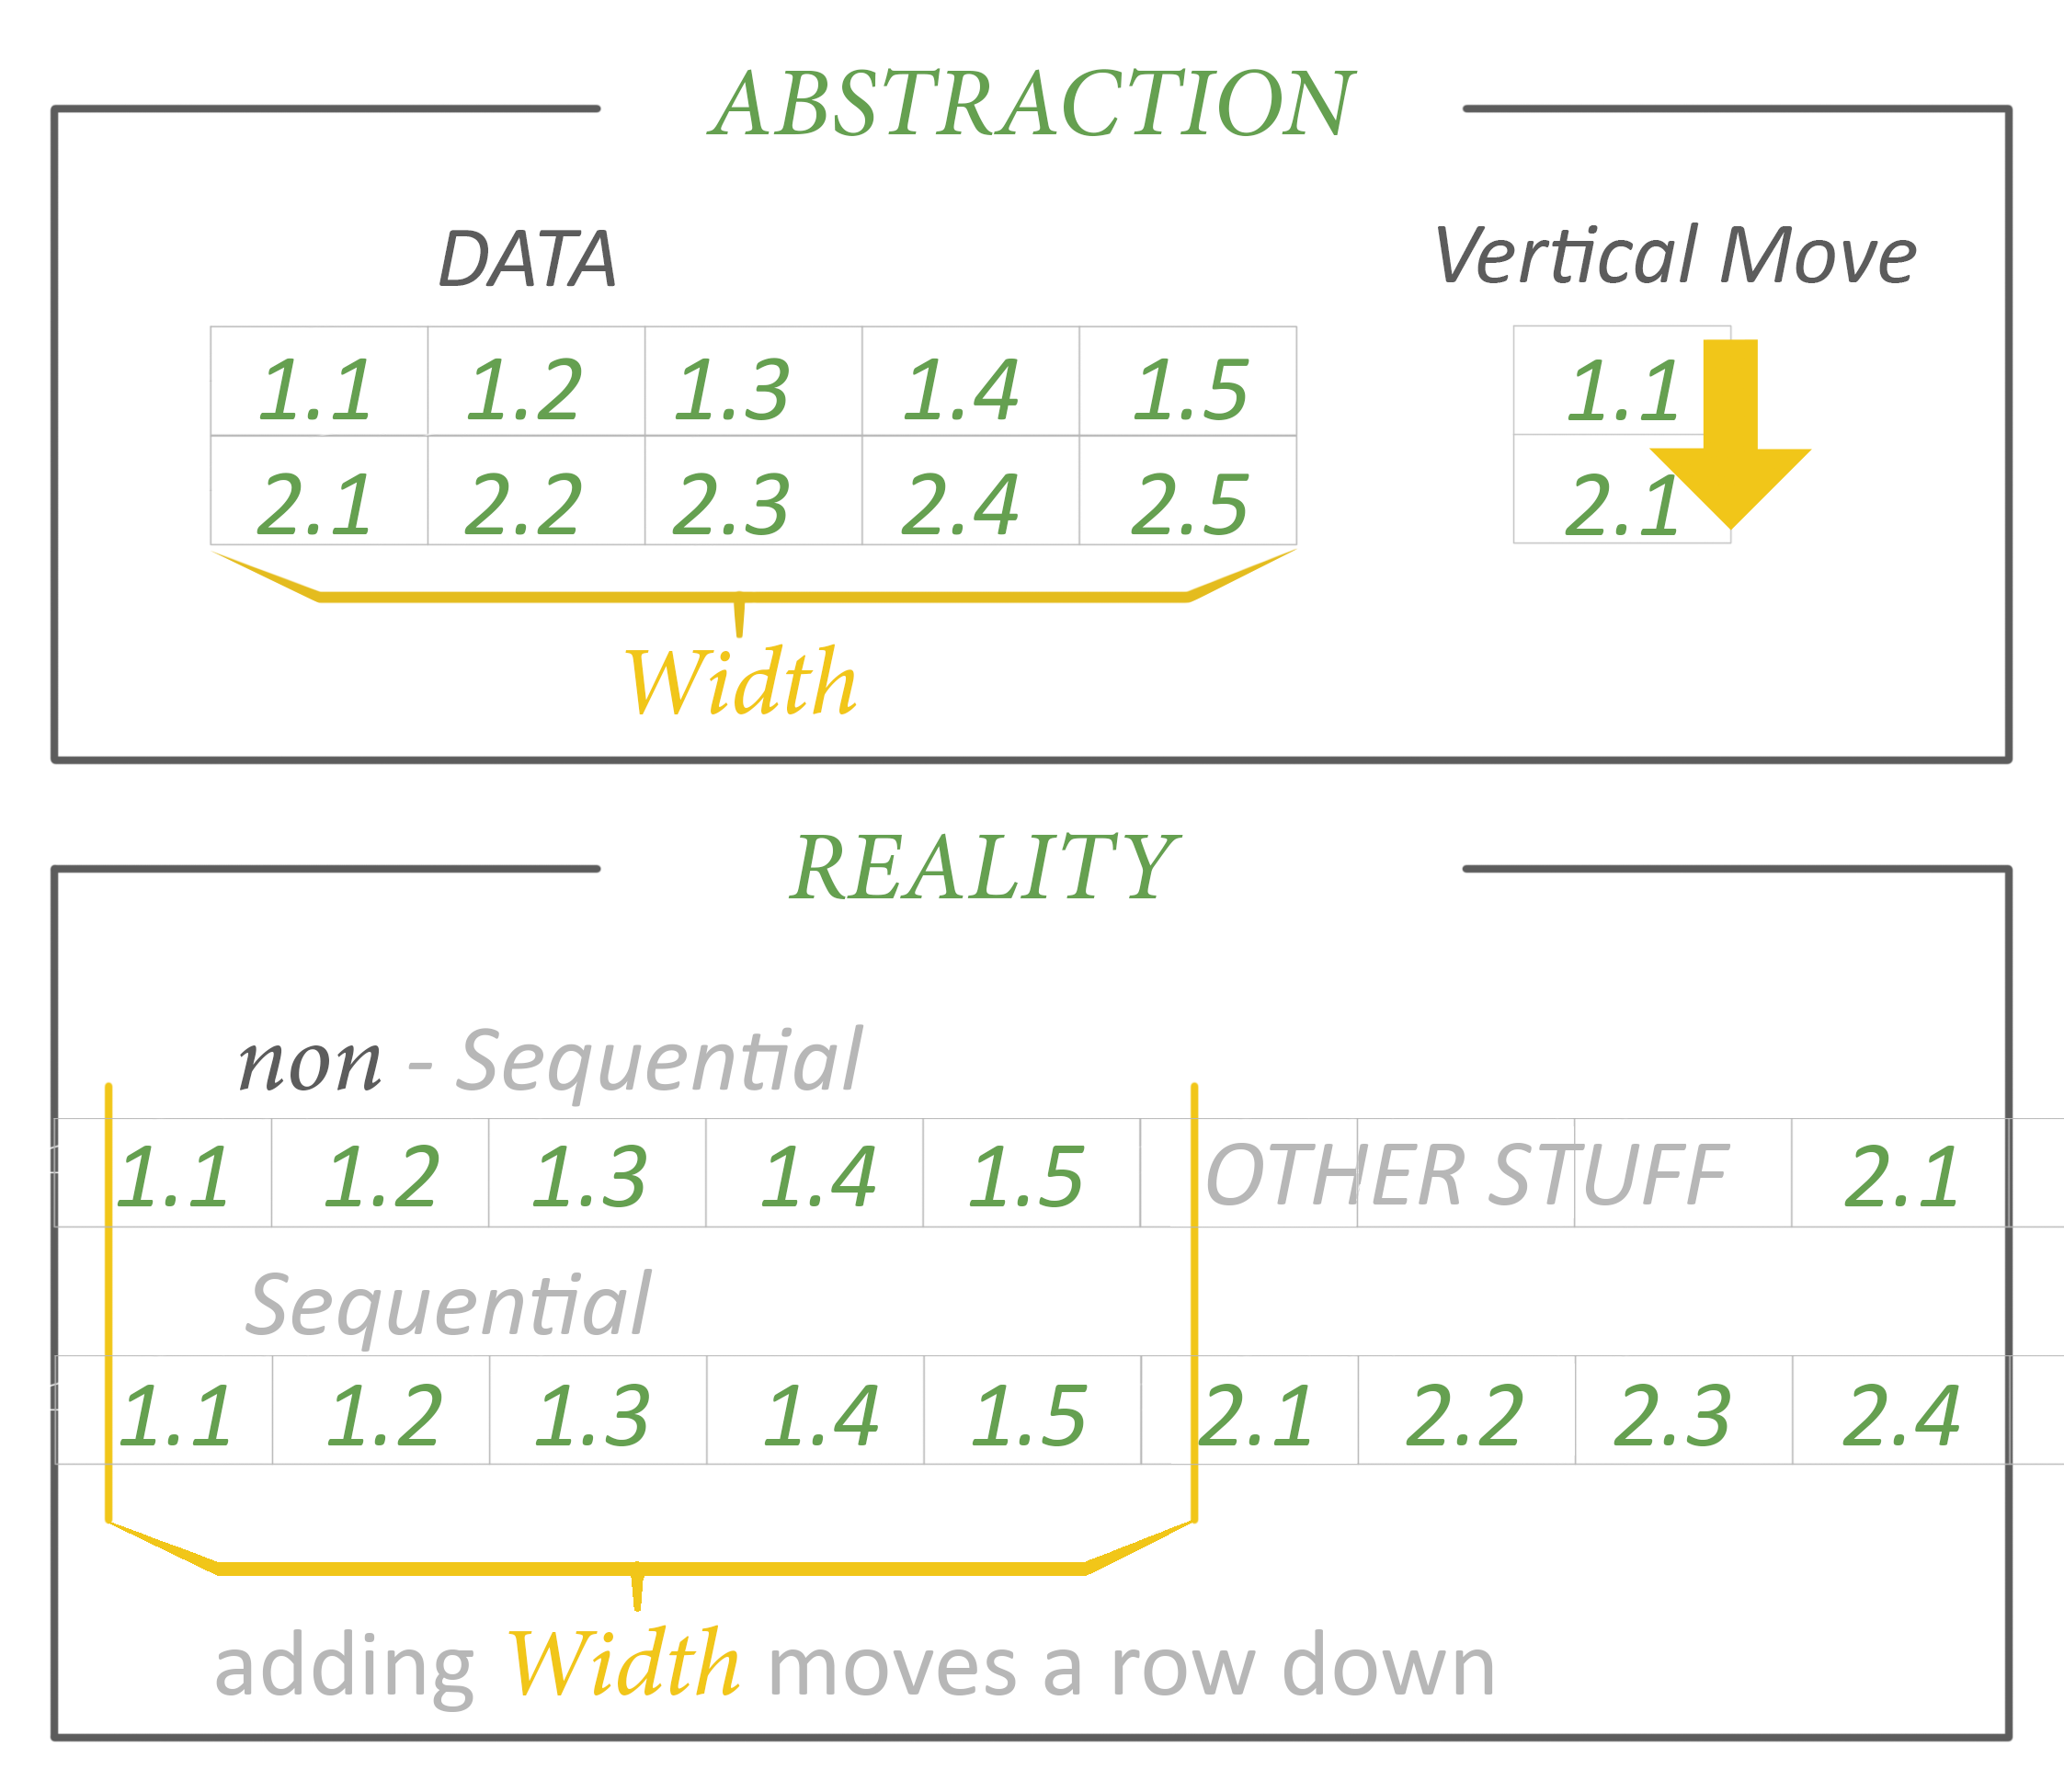
\includegraphics[width=0.6\linewidth]{figure/Analysis/data.png}
	\caption{Visualization of what happens when one adds the images width to a pointer. In a non-sequential image jumping doing this might result in writing to an invalid location. But in a sequentially laid out image it will result in the pointer pointing to the same index in the row below } 
	\label{fig:vis}
\end{figure}
 The implemented method only works if the data in the image is laid out sequentially. Being sequential means that the data of each row is laid out right after each other. So after the last index in the first row, comes the first index in the second row. Normally to get from a coordinate $(x,y)$ to $(x,y+1)$ one would have to get a pointer to the first column using the \codeword{mat.ptr<uchar>(y+1)} and then adding the x value to it. This is exactly what the \codeword{Mat.at<uchar>(y,x)} does. But if the image is sequential one can add the image width to its index and end up in the row below it, as illustrated in \autoref{fig:vis}.\\
 
 Now that we can navigate between pixels, it is possible to implement the algorithm as seen in Listing \ref{listing:grassfireIm}
\begin{listing}[H]
	\caption{The drop fire function starts from one white pixel changes its color and recursively spreads until the entire blob has been consumed. It does this through connected component analysis, analyzing its connected pixels, and spreading to them if they are white.}
	\begin{minted}[frame=lines, framesep=2mm,baselinestretch=1.1,fontsize=\footnotesize,linenos]{c++}
void dropFire(uchar * pixel, glyphObj &store, int &width, int y, int x, cVector &from) {
	*pixel = store.nr;
	from.x = x;
	from.y = y;
	store.list.push_back(from);
	if (*(pixel + GRIDSIZE) == 255) {
		dropFire(pixel + GRIDSIZE, store, width, y, x + GRIDSIZE, from);
	}
	if (*(pixel + width) == 255) {
		dropFire(pixel + width, store, width, y + GRIDSIZE, x, from);
	}
	
	if (*(pixel - GRIDSIZE) == 255) {
		dropFire(pixel - GRIDSIZE, store, width, y, x - GRIDSIZE, from);
	}
	
	if (*(pixel - width) == 255) {
		dropFire(pixel - width, store, width, y - GRIDSIZE, x, from);
	}
}
	\end{minted}
	\label{listing:grassfireIm}
\end{listing} 
The arguments consist of a pointer to the pixel, the blob that this fire is going to add data to, the image's width, two integers that are the fire's current coordinates, and a reference to a vector to avoid instantiating a new one in each recursion. The function starts on line 2 by changing the pixels color to the blobs color, in order to avoid infinite recursion. Lines 3 to 5 adds the current coordinates to the blob. Next are four if statements, each checking if the neighboring pixel in a certain direction are white. If any of them are, it spreads the fire in those directions with the new x and y values.\\

\subsection{Scanning for white pixels}
Scanning for white pixels can be accomplished by looping through each pixel in the image and checking if it is white. This only works if the image is binary. In our case, the image is 8bit gray scale to help visualize the blobs. If the pixel is white, create a blob, add it the list of blobs, and start the fire at the pixel. This is implemented as shown in Listing \autoref{listing:grassfire}.
\begin{listing}[H]
	\caption{Here it is shown how the program scans for white pixels, create blobs if it finds any, and then starts "fires"}
	\begin{minted}[frame=lines, framesep=2mm,baselinestretch=1.1,fontsize=\footnotesize,linenos]{c++}
void grassFireBlobDetection(Mat &biImg, vector<glyphObj> &blobs) {
	int nRows = biImg.rows;
	int nCols = biImg.cols;
	int rowSize = nCols * GRIDSIZE;
	uchar * p;
	uchar * passer;
	glyphObj currentBlob;
	cVector assigner;
	int col = 245;
	for (int i = GRIDSIZE + 1; i < nRows - GRIDSIZE - 1; i += GRIDSIZE) {
		p = biImg.ptr<uchar>(i);
		for (int j = GRIDSIZE + 1; j < nCols - GRIDSIZE - 1; j += GRIDSIZE) {
			if (p[j] == 255) {
				blobs.push_back(currentBlob);
				blobs.back().nr = col;
				passer = &p[j];
				dropFire(passer, blobs.back(), rowSize, i-BORDER, j-BORDER, assigner);
				col -= 10;
				if (col < 20) {
					col = 245;
				}
			}
		}
	}
}
	\end{minted}
	\label{listing:grassfire}
\end{listing}
The arguments for this function are a reference to a binary image, and references to a vector of blobs that will be filled with the data\todo{What data?}. The \codeword{dropFire} function in Listing \ref{listing:grassfireIm} needs to get the images' width, and a variable for this is instantiated on line 4. A temporary blob object(currentBlob), vector(assigner), and uchar pointer(passer) is created to avoid instantiating these objects in the recursive function. A reference to these will be passed instead. Finally the fire's color is set to be 245 in line 9 since it should not be white(255). Inside the double for loop (line 10 to 24) it checks if the current pixel is completely white. If it is, a new blob is added to the vector of glyphObject that contains the blobs, its color is set to the value of col, and the fire starts. To make it easier to display which pixels that belong to which blob, the color is made darker. This means that different fire will "burn" different colors into the image. To prevent the color from becoming negative it is reset when it becomes too dark in line 20 to 23.\\
\begin{figure}[H]
	\centering
	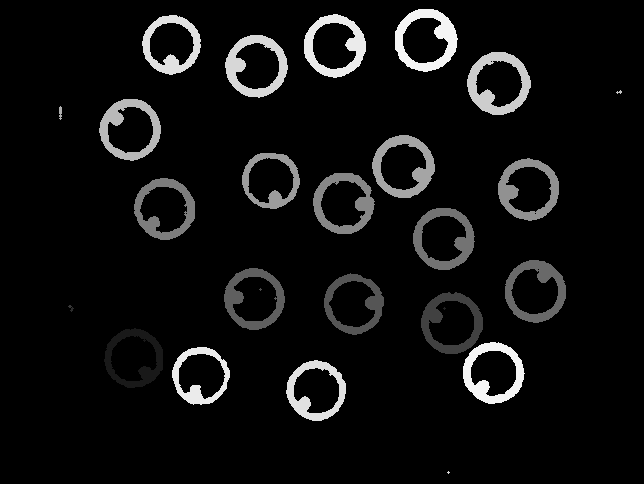
\includegraphics[width=0.6\linewidth]{figure/Analysis/grassfire.png}
	\caption{The test image after the grassfire algorithm has been run. Each blob is made slightly darker than the last one, until a threshold where the color is made white again}
	\label{fig:grsnapshot}
\end{figure} 
The results of the image before and after this algorithm has been run can be seen in \autoref{fig:grsnapshot}. It can be seen that each blob has been segmented from the difference in colors between them. As the color of the fire is changed each time a new fire is started. Then the program must calculate the parameters which are used to evaluate the object.
\todo{What is the purpose of burning 50 shades of gray?}
\section{Blob analysis}
In this section we will describe how to calculate parameters for a given blob, and how these are used to evaluate whether the blob is one of the markers.
\subsection{Parameter overview, and flow}
A blob is determined to be a marker by considering the following parameters:
\begin{enumerate}
	\item Number of pixels in the blob.
	\item Height to width relationship of the bounding box.
	\item Bounding box center.
	\item Rotation of the blob.
\end{enumerate}
When all parameters are acquired, and if the blob passes all the tests, it is time to check the value in the glyph. To do this, vectors are calculated based on the rotation that sample a pixel in each "bit" in the glyph and calculate the total value of it. If this value is between 1 and 255 it is considered a marker, and this blob is flagged so it can be sent to unity. The flow chart of each blob is analyzed can be seen in Figure \ref{fig:flow}.

\begin{figure}[H]
	\centering
	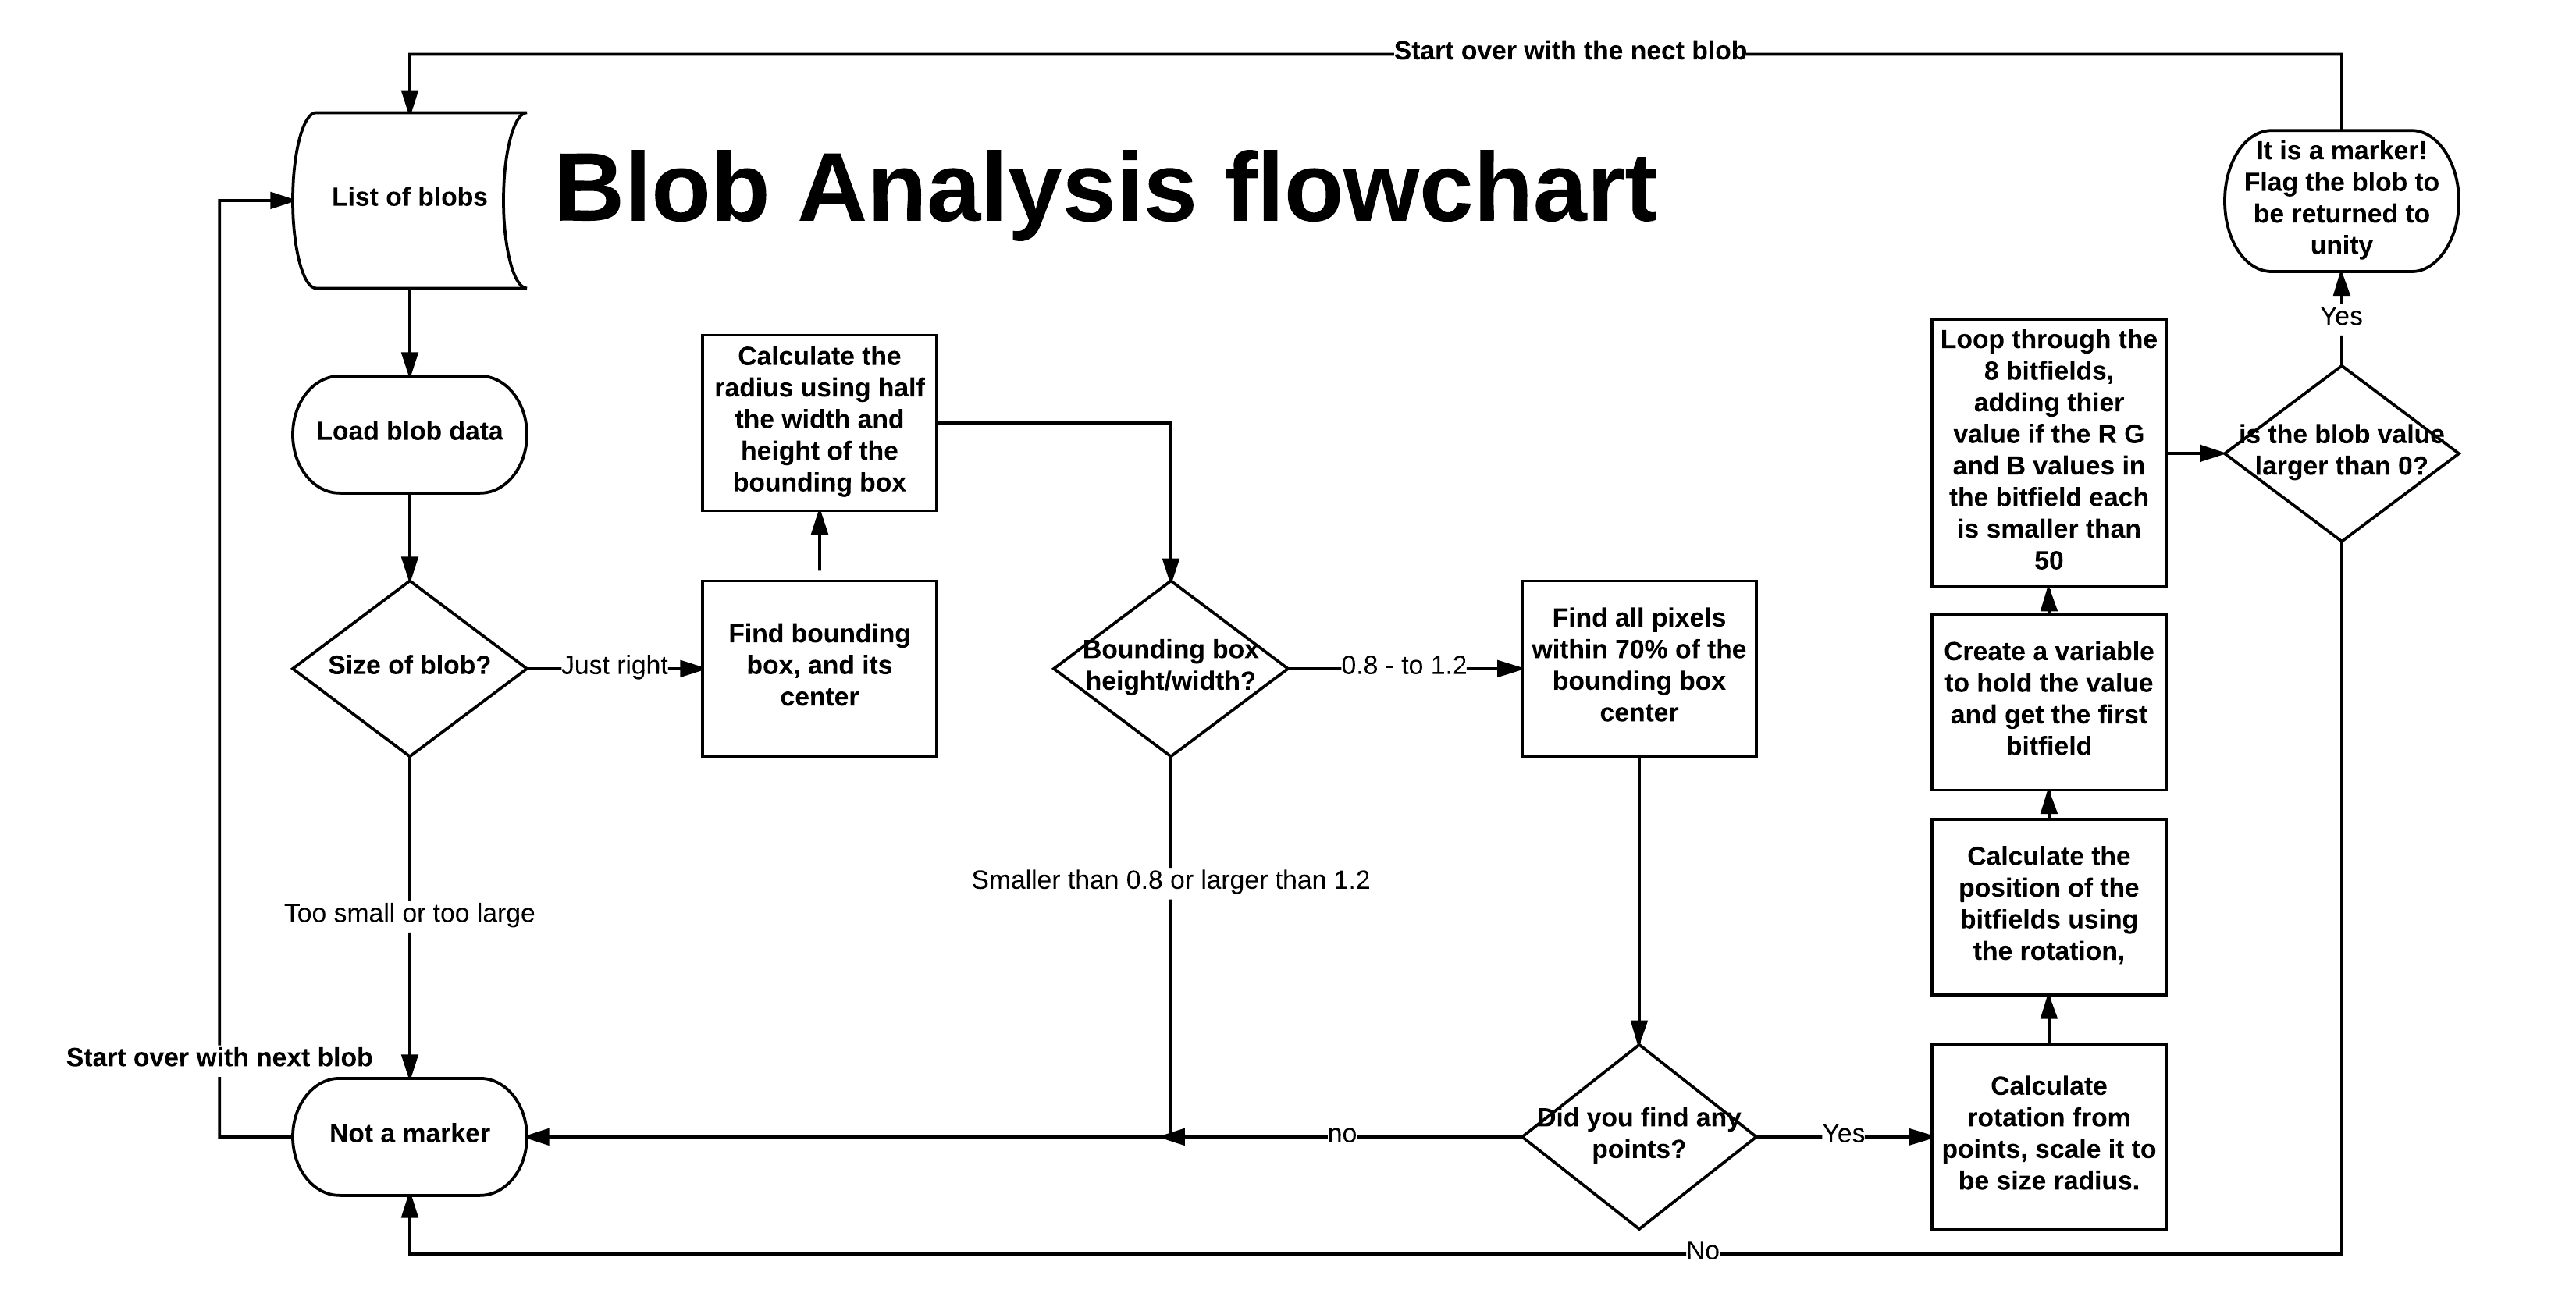
\includegraphics[width=1\linewidth]{figure/Analysis/flowchart.png}
	\caption{The flow chart of the blob analysis algorithm, showing how we determine whether the returnable variable in each blob should be set to true. This decide which blobs get sent to Unity}
	\label{fig:flow}
\end{figure} \todo{this is hard to read, change size of picture i guess??}
In regards to calculating the parameters, some of them are very simple to find. Finding the number of pixels of a blob is easy because \codeword{vector<type>} already contains a \codeword{.size()} method. The bounding box consists of looping through all coordinates and saving the smallest and largest x and y that the program encounters. Finding the center consists of averaging the same values for x and y respectively. Rotation, on the other hand is trickier and requires knowledge of the layout of the marker.
  
\subsection{Rotation}
Finding a circle's rotation is impossible if it is rotationally symmetrical. A small line was added towards the center that will be referred to as the direction line(seen to the left in Fig \ref{fig:vector}). If the center's coordinates are known, one can find the pixel in the blob closest to it. This pixel will be in the direction line. The distance from the center to the closest pixel will give create a vector, from which the rotation can be calculated. This method of finding rotation is the primary reason why we used the bounding box center over center of mass when finding the center. The center of mass would be shifted towards the rotation line, and therefore the direction vector will be less stable, as illustrated in Figure \ref{fig:boundbox}.\\
\begin{figure}[H]
	\centering
	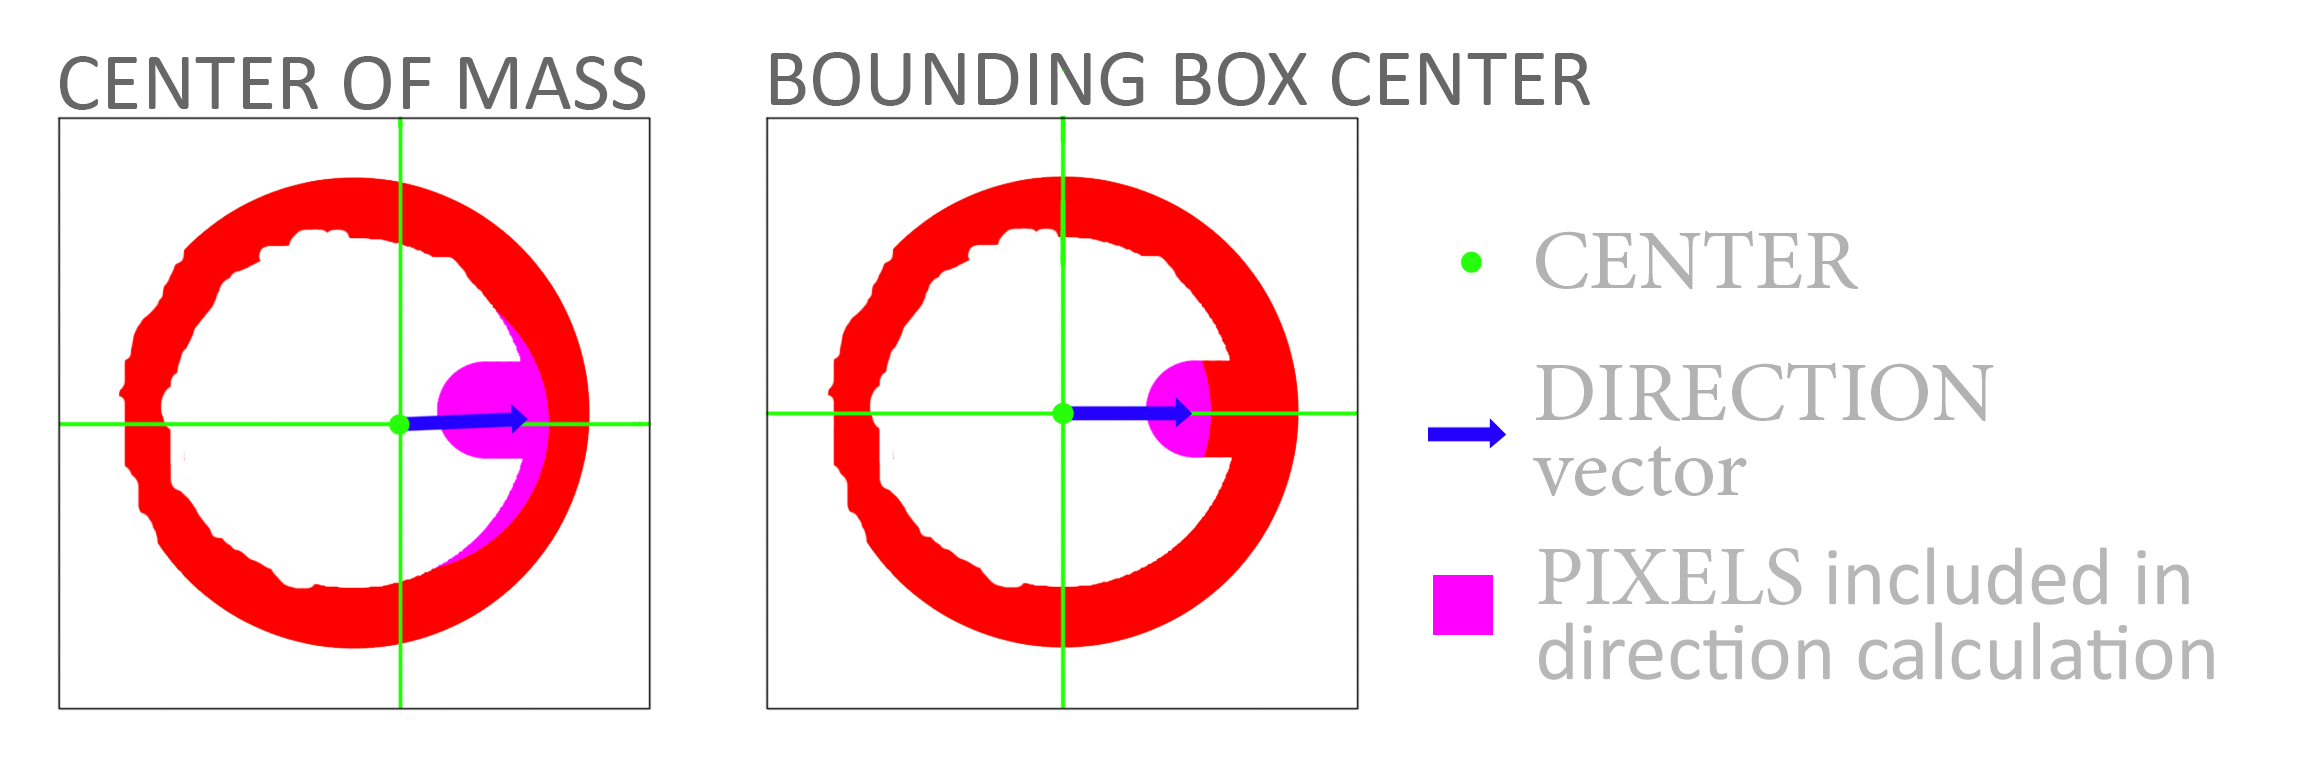
\includegraphics[width=1\linewidth]{figure/Analysis/boundingbox.png}
	\caption{The difference between using the center of mass or bounding box to find the blob center. With bad thresholding the found center is closer to the actual center, resulting in a better direction vector} 
	\label{fig:boundbox}
\end{figure}
We found that smaller blobs would have a more wobbly direction vector, because their direction line contains fewer pixels. Since it only finds one pixel it could result in a drastic snap. To combat this, instead of only using the closest pixel, we average all the pixels within 70\% of the circles radius. This allows us to average a bunch of pixels in the direction line without sampling any from the
periphery. Rotation is also calculated as a float instead of integer. These changes make the direction vector much more stable, and have been illustrated in Figure \ref{fig:lowpixel}
\begin{figure}[H]
	\centering
	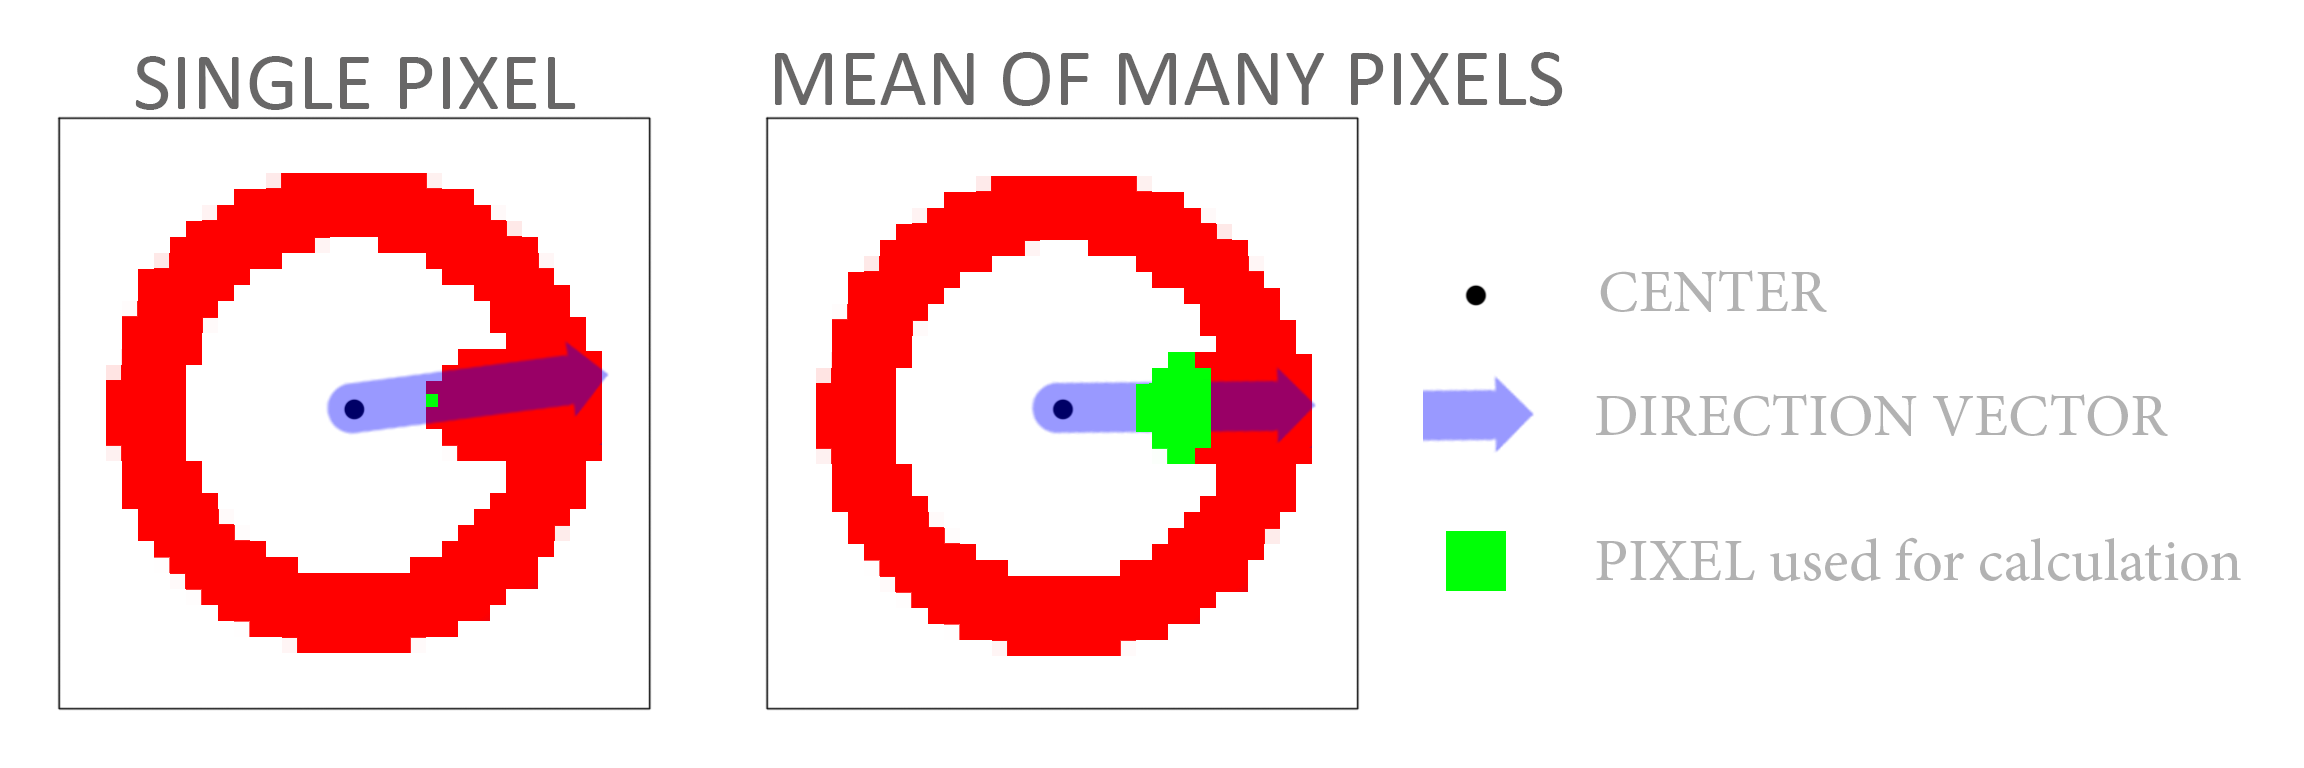
\includegraphics[width=1\linewidth]{figure/Analysis/lowpixel.png}
	\caption{Illustration of the advantage of using mean of many pixels over using the single closest pixel to calculate the direction vector.} 
	\label{fig:lowpixel}
\end{figure}
 The code, seen in listing \ref{listing:direction}, executes inside a loop through the list of blobs, right after the bounding box and its center has been found. \codeword{i} refers to the current blob.
 \todo{Describe here what the code actually does. Also line 10 has a comment that is missing something}
\begin{listing}[H]
	\caption{Direction vector calculation}
	\begin{minted}[frame=lines, framesep=2mm,baselinestretch=1.1,fontsize=\footnotesize,linenos]{c++}
float heightWidth = ((largestX - smallestX) / (float)(largestY - smallestY));
//check: discriminate based on height width relation
if (heightWidth > (1 + discrimHW) || heightWidth <(1 - discrimHW)) { continue; }	

radiusDist = (largestX - smallestX + largestY - smallestY) / 4;
searchDist = (float)radiusDist*0.70 * (float)radiusDist*0.70;
int dist;
vector<cVector> points;  //contains the pixels within 0.7 radius
//find pixel within search dist
for (auto &v : i.list) {	//loop through all pixels in the
	dist = (v.x - i.center.x) * (v.x - i.center.x) + (v.y - i.center.y) * (v.y - i.center.y);
	if (dist < searchDist) {
		points.push_back(v);
	}
}
float rotX = 0;
float rotY = 0;
for (auto &p : points) {
	rotX += p.x - centerX;
	rotY += p.y - centerY;
}
rotX = (rotX / points.size());
rotY = (rotY / points.size());
	\end{minted}
	\label{listing:direction}
\end{listing}
Now that a direction vector has been found, we need to calculate the position of each bit field on the marker. This is done with vector math and knowledge of the marker layout. A legend of the important components can be seen in Figure \ref{fig:vector}.

\subsection{Vectors to find sample points}
The direction vectors' length will vary a bit, as sometimes the middle point will move a pixel or two. Under these circumstances the direction vector will still be reasonably stable, but its length will change depending on how much of the direction line is used for the direction calculation. Ideally the vectors would be based on a more stable property of the marker. For this reason, the direction vector is scaled so that its length is equal to the radius. We can now define distances as percentages of the markers radius. Sample points are the point where we check image intensity to determine whether the field is white or dark. These can be thought of as points on a "skeleton" made up of different vectors, as shown in \autoref{fig:vector}.
\begin{figure}[H]
	\centering
	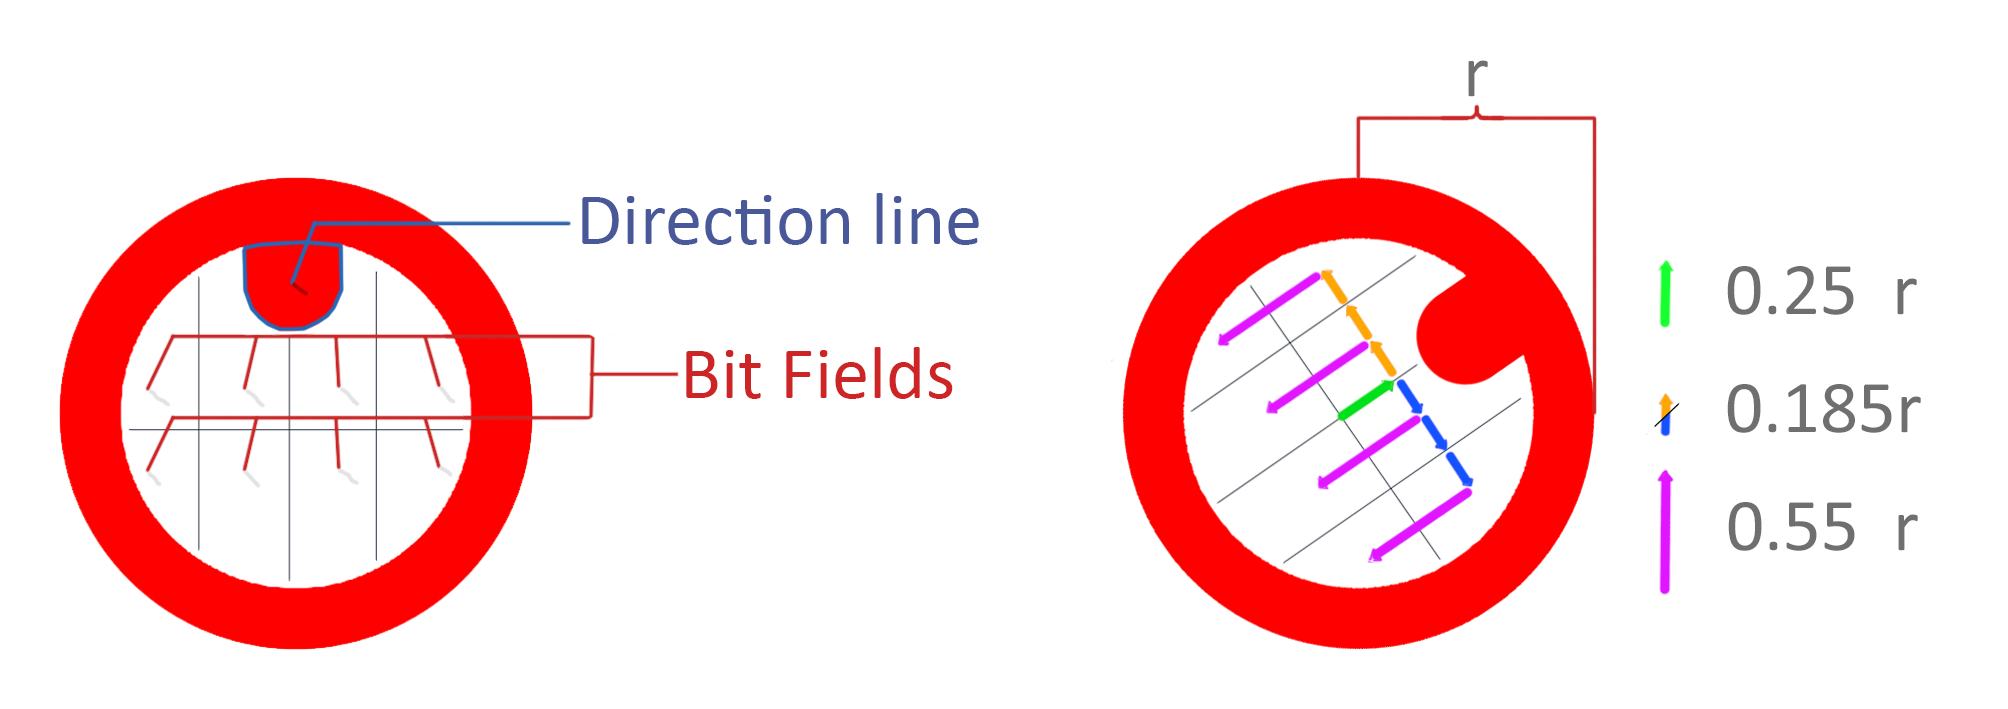
\includegraphics[width=1\linewidth]{figure/Analysis/vector.png}
	\caption{To the left one can see the location of the direction line, used to find the direction that the marker is facing, and the bit fields used to ascertain the marker's value. To the right, the "skeleton" of vectors used to find bit fields coordinates are shown.} 
	\label{fig:vector}
\end{figure}
Finding the sample points is a matter of adding the correct vectors to the marker's center. To begin a start point is created 25 percent towards the direction line. From here there are three different types of vector used to reach the sample points: Two that move perpendicular to the direction, used to move "sideways", and one that moves opposite the direction to get the second row of points. Rotating a vector 90° is fortunately easy, and can be done by flipping the axis and changing a sign(- x, or -y).    
\begin{listing}[H]
	\caption{Declaration of vectors used to find sample points}
	\begin{minted}[frame=lines, framesep=2mm,baselinestretch=1.1,fontsize=\footnotesize,linenos]{c++}
	int startPointX = centerX + rotX*0.25;
	int startPointY = centerY + rotY*0.25;
	
	//Perpendicular movement
	float cClockX = -rotY*0.185;
	float cClockY = rotX*0.185;
	float clockX = rotY*0.185;
	float clockY= -rotX*0.185;
	
	//Backwards movement
	float reverseX = -rotX*0.55;
	float reverseY = -rotY*0.55;
	\end{minted}
	\label{listing:vectors}
\end{listing}
From these, the sample points can be acquired and the program can check whether the bit fields that they point to are dark or white. This is done by checking each color in the original image and, if they all are below a threshold, adding 2 to the power of the field to the total count, which is the number that identifies a marker. The implementation can be seen in Listing \ref{listing:sumingval}.
 \begin{listing}[H]
 	\caption{After finding the sample points, this code checks the value in that pixel and, if low enough, adds its value to the bit counter. If the bit counter is larger than 0 when all points have been checked, the bit counter is assigned to the blob's nr variable, allowing it to be returned to Unity.}
 	\begin{minted}[frame=lines, framesep=2mm,baselinestretch=1.1,fontsize=\footnotesize,linenos]{c++}
int bitCounter = 0;					//total marker value
int thresh = 50;
for (auto &sp : searchPoints) {		//loop through each point
	Vec3b intensity = drawImg.at<Vec3b>(sp.y, sp.x);
	if (intensity[0]< thresh && intensity[1] < thresh && intensity[2] < thresh) {
		bitCounter += pow(2, iterations);
	}
}

if (bitCounter > 0) {
	i.returnable = true;
	i.nr = bitCounter;
}
 	\end{minted}
 	\label{listing:sumingval}
\end{listing}
Finally, since human skin captured by the webcam often returns a false positive marker with total count value 0, the object is not returned to Unity unless at least one of the bit fields are dark.
So finally we can present the final image after the blobs have been analyzed. 
\begin{figure}[H]
	\centering
	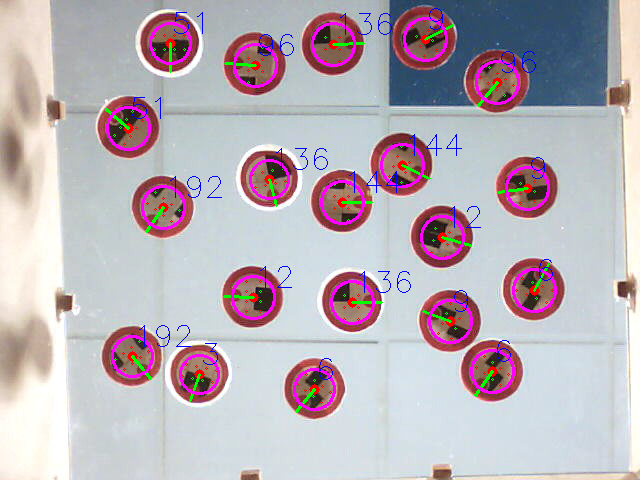
\includegraphics[width=1\linewidth]{figure/Analysis/output.png}
	\caption{The output after the blobs have been analyzed. The circle whose radius is used to find points for the direction vector is drawn in magenta. The direction vector after scaling it to have a length of radius is drawn in green. The sample points are drawn in either red, if they are white, or green if they are considered dark} 
	\label{fig:output}
\end{figure}

Returning the objects to Unity is simple. 
 \begin{listing}[H]
	\caption{Returning all blobs that have passed the test to Unity}
	\begin{minted}[frame=lines, framesep=2mm,baselinestretch=1.1,fontsize=\footnotesize,linenos]{c++}
for (auto &blob : blobs) {
	if (outDetectedMarkersCount == maxOutMarkersCount)	break;
		if (blob.returnable == false)	continue;
		
		rotation = acos(blob.rotation.x / sqrt((blob.rotation.x * blob.rotation.x)
		 + (blob.rotation.y * blob.rotation.y)));
		outMarkers[outDetectedMarkersCount] = 
		ObjectData(screenWidth - blob.center.x, screenHeight - blob.center.y
		, blob.nr, blob.rotation.x, blob.rotation.y, (180 / 3.1415) * rotation);
		outDetectedMarkersCount++;
}
	\end{minted}
	\label{listing:return}
\end{listing}

\todo{Explain the above code}

\section{Unity}
	Continuing from Listing \ref{listing:pointer},\todo{What does this mean? Rephrase.} we now have the means to add the markers to an array of CVObjects called \codeword{_markers}. When the script starts, the \codeword{Detect()} function runs every second, using \codeword{InvokeRepeating()}. The detect function in Listing \ref{listing:detectFunction} clears the elements array, which is what holds the \codeword{GameObjects}. By making the pointer \codeword{outMarkers} we can directly change the contents of \codeword{_markers} to be whatever markers the image processing function finds. When declaring the pointer to \codeword{_markers}, we also use that pointer at line 10 in Listing \ref{listing:detectFunction}, passing the newly made pointer into C++. \codeword{unsafe} is added to enable the use of pointers inside C\#, and \codeword{fixed} ensures the function stays at the same location of the memory.
	\begin{listing}[H]
		\caption{C\# function that receives the markers from the DLL file.}
		\begin{minted}[frame=lines, framesep=2mm,baselinestretch=1.1,fontsize=\footnotesize,linenos]{csharp}
private void Detect(){
	if (shouldDetect) {
		if (elements.Capacity > 0) {
			clearElements();
		}
		elements = new List<GameObject>();
		int detectedMarkersCount = 0;
		unsafe{
			fixed (CVObject* outMarkers = _markers) {
				Cap(outMarkers, _maxMarkerDetectCount, ref detectedMarkersCount);
			}
		}
		for (int i = 0; i < _markers.Length; i++) {
			Spawn(_markers[i].Type, _markers[i].X, _markers[i].Y,
			_markers[i].Rotation, _markers[i].RotationY);
		}
	}
}
	\end{minted}
\label{listing:detectFunction}
\end{listing}
Then we loop through the \codeword{_markers} array and spawn the appropriate object for each one. The type of object is determined in Listing \ref{listing:sumingval}, and rotation is calculated in Listing \ref{listing:direction}.\\

The spawn function in Listing \ref{listing:spawnFunction} makes a new \codeword{GameObject} from the arguments passed to it. If $x == 0$ and $z == 0$ then we default the type to be -1, which means that it is a false positive and may be discarded. If the Y rotation is above 0, the rotation should be flipped, as the rotation can only be between 0 and 180. Hence, to get the full 360 rotation needed to fully rotate the object in virtual space, it is made to rotate the other way.
\begin{listing}[H]
	\caption{C\# function that spawns the objects in the world, and add them to the elements array.}
	\begin{minted}[frame=lines, framesep=2mm,baselinestretch=1.1,fontsize=\footnotesize,linenos]{csharp}
private void Spawn(int type, int x, int z, int rotation, int rotationY) {
	if (x == 0 && z == 0) { type = -1; }
	if (type != -1 && type != 0) {
		if (rotationY > 0) {
			rotation *= -1;
		}
		GameObject tempObj = Instantiate(FindObj(type), PositionGen(x, z),
		Quaternion.Euler(\\
		 rotation, 0)) as GameObject;
		elements.Add(tempObj);
	}
}
	\end{minted}
\label{listing:spawnFunction}
\end{listing}
The \codeword{FindObj()} function is simply a switch case that returns the correct object from the number passed to it. The \codeword{PositionGen()} function returns the given position divided by 25, which is required to make the objects fit in the virtual garden. The element is added to the elements array, making it so that the objects can be cleared again for the next pass which follows immediately after.

